\section*{Anhang}

\begin{frame}
\begin{figure}
	\centering
	\begin{subfigure}{.85\textwidth}
	\centering
	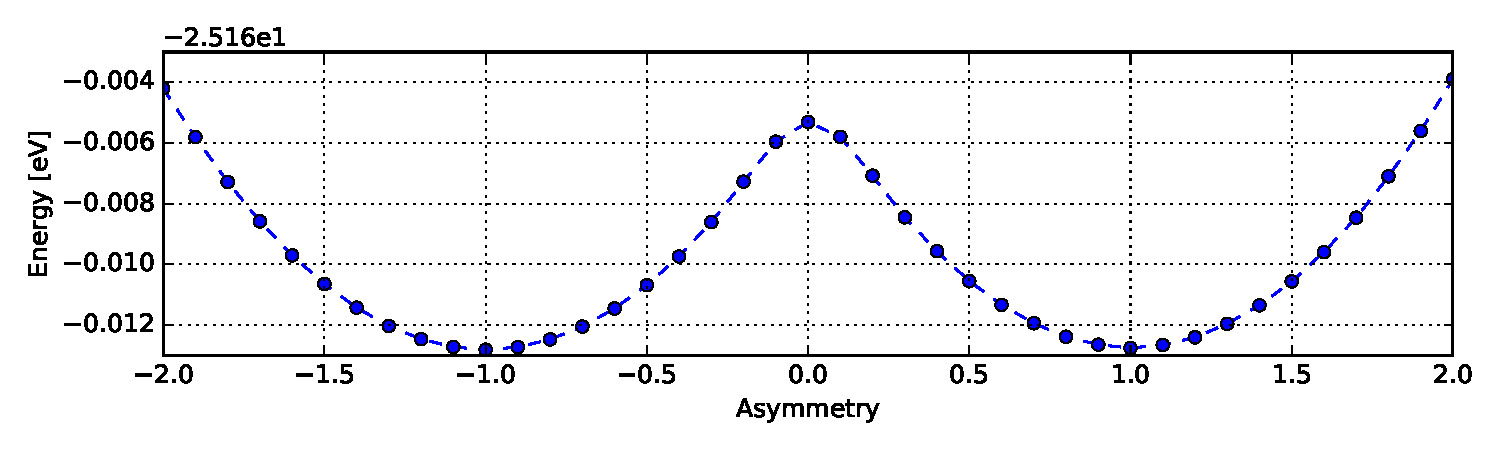
\includegraphics[width = \textwidth]{Images/polyacetylene/convergence/Potential_with_asymmetry}
	\caption{Mit $k$-Punkt am \textsc{Brillouin}-Zonen-Rand.}
	\label{image_potential_with_asymmetry}
	\end{subfigure}
	\begin{subfigure}{.85\textwidth}
	\centering
	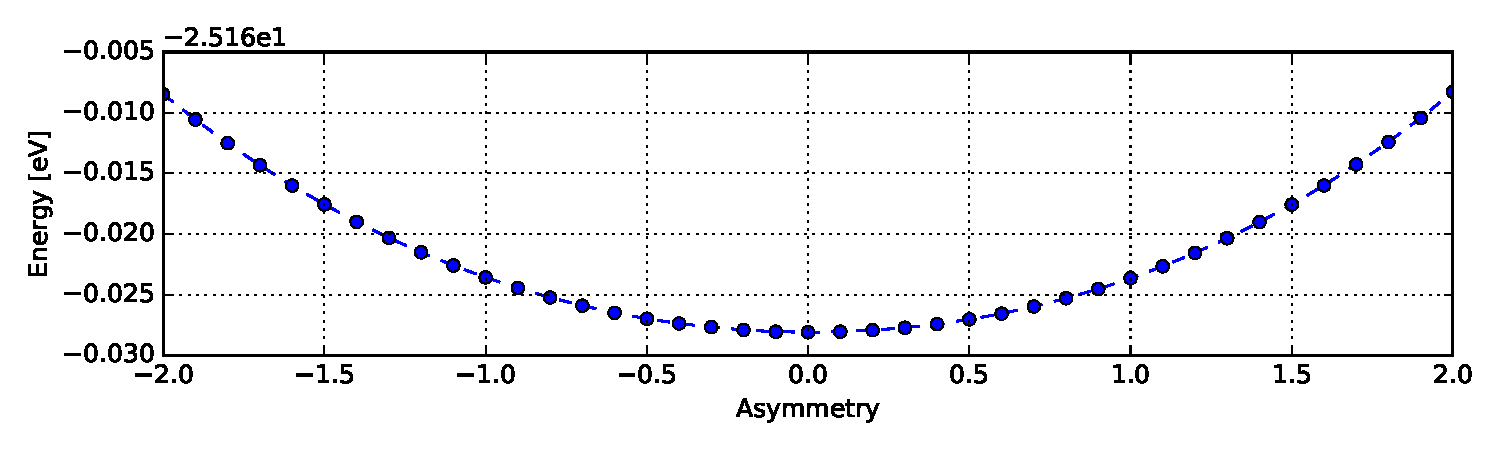
\includegraphics[width = \textwidth]{Images/polyacetylene/convergence/Potential_without_asymmetry}
	\caption{Ohne $k$-Punkt am \textsc{Brillouin}-Zonen-Rand.}
	\label{image_potential_without_asymmetry}
	\end{subfigure}
	\caption{Grundzustandsenergie in Abhängigkeit von der Asymmetrie $\nicefrac{u}{u_0}$.}
\end{figure}
\end{frame}

\begin{frame}
\begin{figure}
\centering
\begin{tikzpicture}[show background rectangle, scale = .65]
	\foreach \x in {0,...,7}{
		\draw[line width=1pt] (\x,0) .. controls (\x + 1, 2) and (\x - 1 , 2) .. cycle .. controls (\x + 1, -2) and (\x - 1 , -2) .. cycle;
	}
	\foreach \x in {0, 4}
	\foreach \y in {0, 1}
	\foreach \z in {-1, 1}
	\node at (\x + \y - \z + 1, \z) {\large +};
	\foreach \x in {0, 4}{
		\foreach \y in {0, 1}{
			\foreach \z in {-1, 1}{
				\node at (\x + \y - \z + 1, -\z) {\large -};
	}}}
	\draw[line width = 0.2] (-0.1, -1.8) -- +(-0.3, 0) -- +(-0.3 ,3.6) -- +(0,3.6);
	\draw[line width = 0.2] (1.1, -1.8) -- +(0.3, 0) -- +(0.3 ,3.6) -- +(0,3.6);
	\draw[line width = 0.2] (3.9, -1.8) -- +(-0.3, 0) -- +(-0.3 ,3.6) -- +(0,3.6);
	\draw[line width = 0.2] (7.1, -1.8) -- +(0.3, 0) -- +(0.3 ,3.6) -- +(0,3.6);
	\draw[dotted, line width = 1.5] (-0.6,0) -- (-1,0);
	\draw[dotted, line width = 1.5] (7.6,0) -- (8,0);
\end{tikzpicture}
\caption{Schema: p-Orbitale von alternierender $\pi$-Bindung.}
\end{figure}
\begin{figure}[]
	\centering
	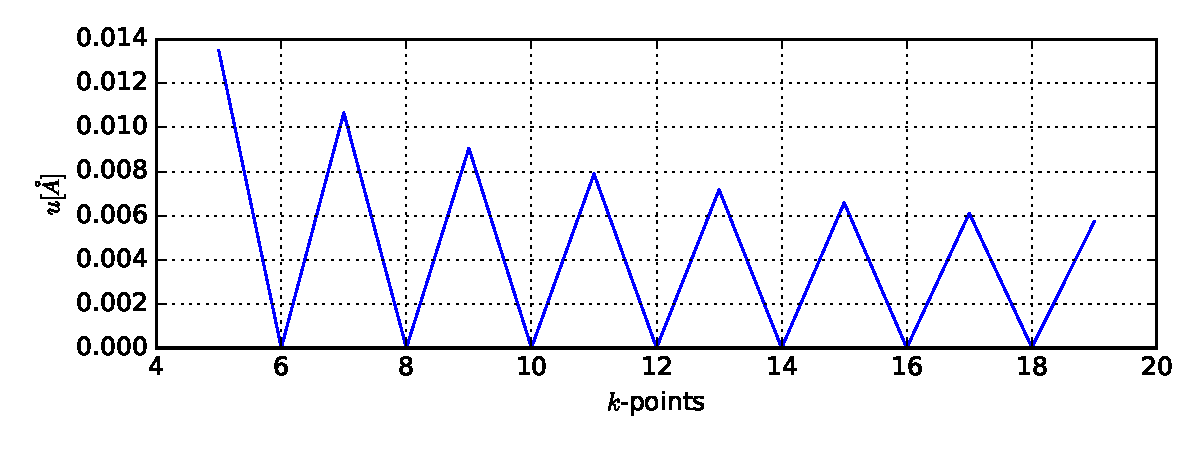
\includegraphics[width = .7\textwidth]{Images/polyacetylene/convergence/displacement_double_cell_poly}
	\caption{Verschiebung $u$ in Abhängigkeit von den $k$-Punkten für eine Einheitszelle mit vier CH-Gruppen.}
	\label{image_disp_double_cell_poly}
\end{figure}
\end{frame}

\begin{frame}
\begin{figure}
	\centering
	\begin{subfigure}{0.25\textwidth}
		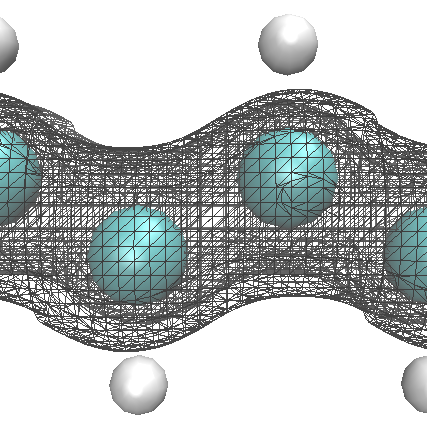
\includegraphics[width = \textwidth]{Images/polyacetylene/wavefunctions/Mid_band_2_Cut}
		\caption{Bindend}
		\label{image_homo1}
	\end{subfigure}\hspace*{2cm}
	\begin{subfigure}{0.41\textwidth}
		\centering
		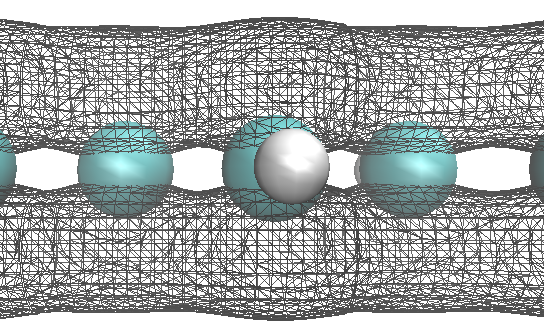
\includegraphics[width = \textwidth]{Images/polyacetylene/wavefunctions/Mid_band_2_Side_View_Cut}
		\caption{Bindend Seitenansicht}
		\label{image_lumo1}
	\end{subfigure}
	\begin{subfigure}{\textwidth}
		\centering
		\begin{tikzpicture}[show background rectangle, yscale = .6]
		\foreach \x in {0,...,7}{
			\draw[line width=1pt] (\x,0) .. controls (\x + 1, 2) and (\x - 1 , 2) .. cycle .. controls (\x + 1, -2) and (\x - 1 , -2) .. cycle;
		}
		\foreach \x in {0,...,7}{
			\foreach \y/\s in {-1/+, 1/-}{
				\node at (\x, \y) {\large \s};}}
		\draw[dotted, line width = 1.5] (-0.6,0) -- (-1,0);
		\draw[dotted, line width = 1.5] (7.6,0) -- (8,0);
		\end{tikzpicture}
		\caption{Schema: p-Orbitale am $\Gamma$-Punkt}
		\label{image_homo1_side_view}
	\end{subfigure}
	\caption{Isooberflächen für Zustände am $\Gamma$-Punkt.}
\end{figure}
\end{frame}

\begin{frame}
\begin{itemize}
	\item Perfekt, periodische Kette:
	\begin{align*}
	\mathcal{H} &= \sum_i E_0 n_i - \sum_i t \left(c_i^\dagger\  c_{i+1} + c_{i+1}^\dagger\  c_i\right)
	\end{align*}
	\item Eigenenergien: $E_k = E_0 \pm \underbrace{2t\cos(ka)}_{=:\epsilon_k}$
\end{itemize}
\begin{figure}
	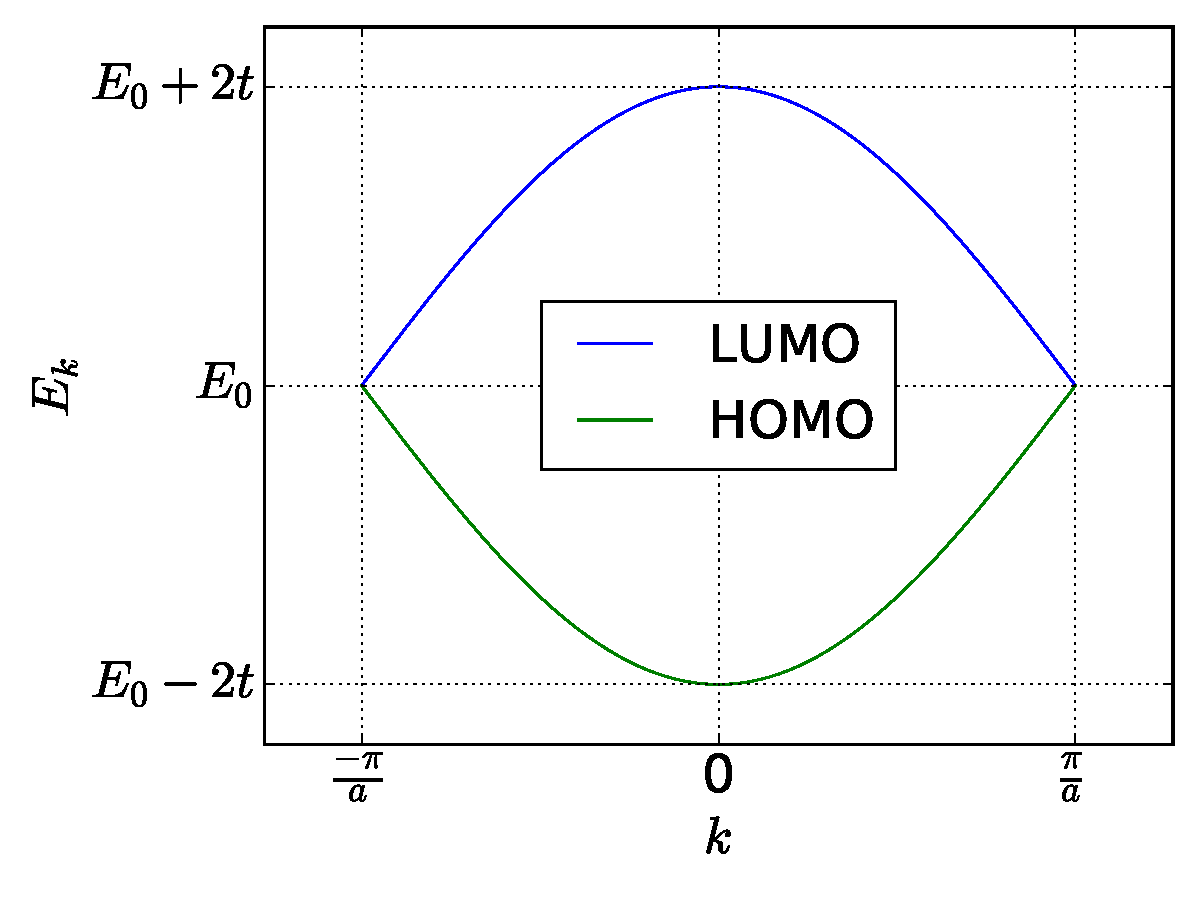
\includegraphics[width =0.6\textwidth]{Images/Plots/bandstructure_symmetric}
\end{figure}
\end{frame}

\begin{frame}
\frametitle{Bandstruktur}
\begin{align*}
\mathcal{H}_\text{hopp} &= -2\sum_n \left[t_0 + (-1)^n\delta\right]\cdot\left(c_{n+1}^\dagger c_n + c_n^\dagger c_{n+1}\right)\\
&\Downarrow\text{Fourier-Transformation}\\
\mathcal{H}_\text{hopp} &= \sum_k \underbrace{\left[
	\left(\epsilon_k + i\Delta_k\right)c_{k}^{\dagger(e)}c_{k}^{(o)} + \left(\epsilon_k-i\Delta_k \right)	c_{k}^{\dagger(o)}c_{k}^{(e)}\right]}_{\mathcal{H}_k}
\end{align*}
Mit $\epsilon_k := 2t_0\cos(ka)$ und $\Delta_k := 2\delta\sin(ka)$\\
\begin{align*}
E_k &= \pm \sqrt{\epsilon_k^2+\Delta_k^2}
\label{equation_energy_band}
\end{align*}
\end{frame}

\begin{frame}
\begin{figure}
	\centering
	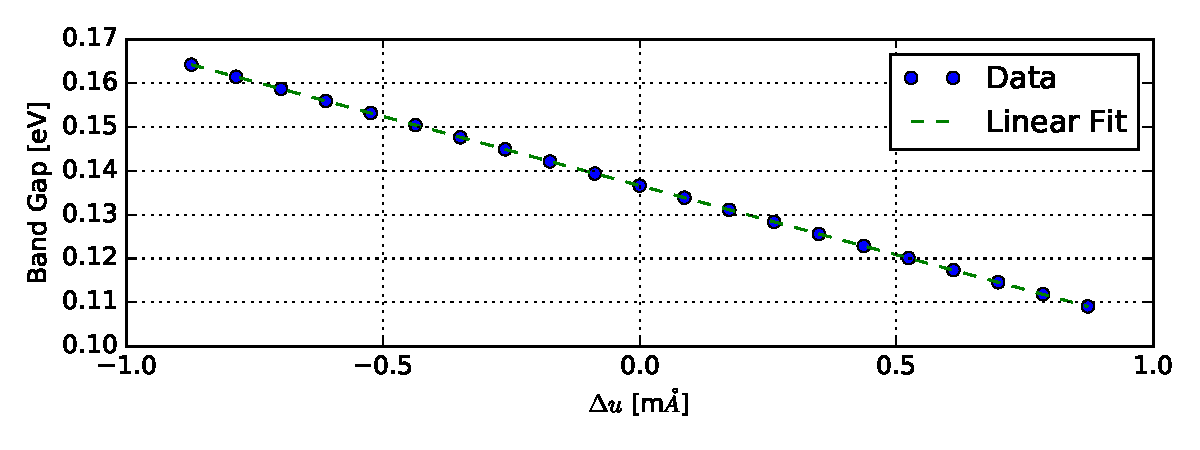
\includegraphics[width = 9cm]{Images/polyacetylene/bands/alpha}
	\caption{Bandlücke in Abhängigkeit von der Verschiebung.}
	\label{image_alpha_fit}
\end{figure}
\end{frame}

\begin{frame}
\begin{figure}
\centering
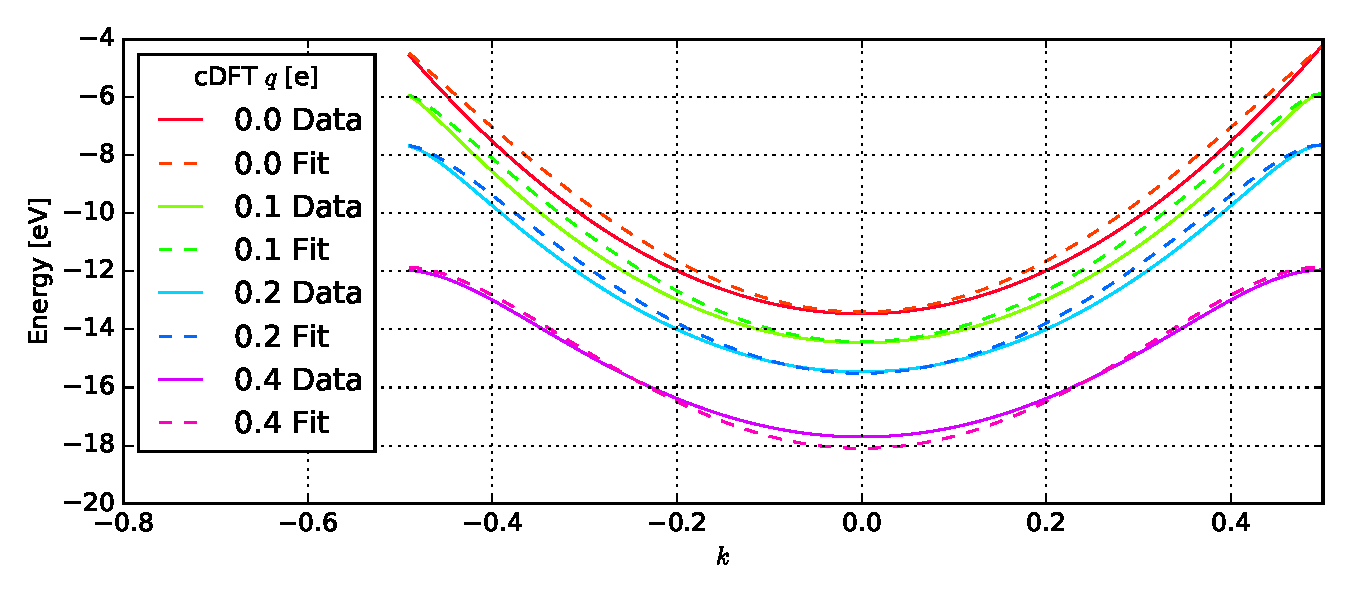
\includegraphics[width = 8cm]{Images/Hydrogen/charging/3D_cuts}
\caption{Wasserstoff-Kette}
\label{image_hydrogen_3D_slices}
\end{figure}
\vspace*{-.7cm}
\begin{figure}
\centering
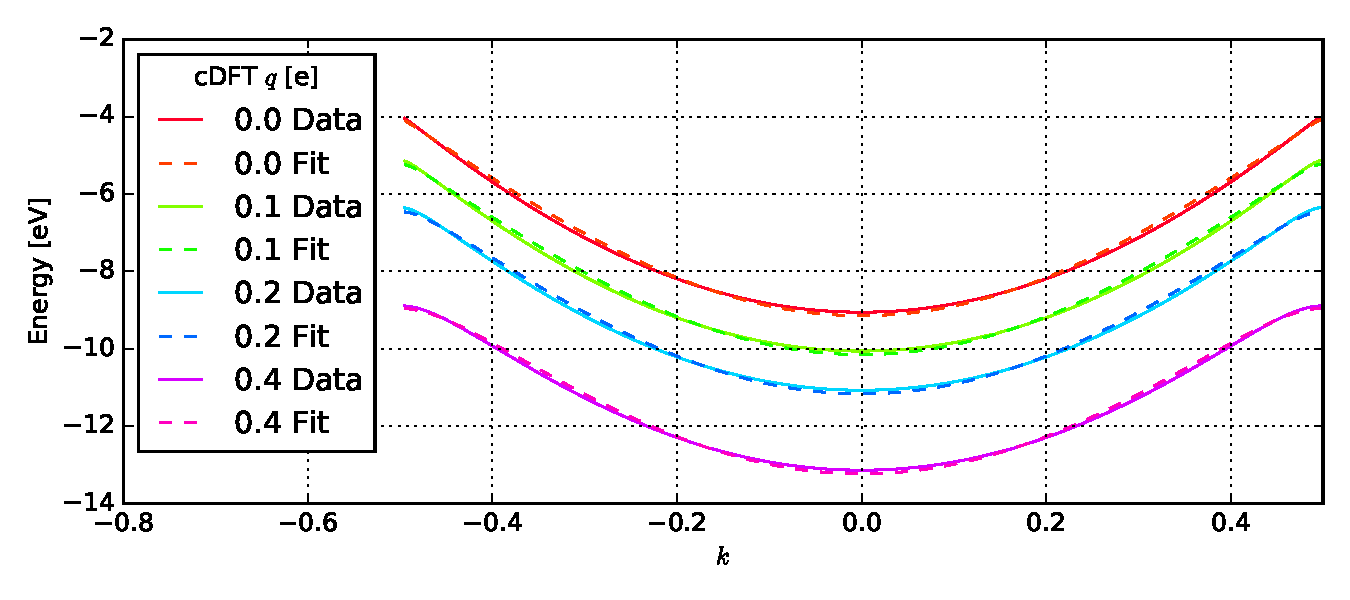
\includegraphics[width = 8cm]{Images/polyacetylene/charging/3D_cuts}
\caption{\emph{trans}-Polyacetylen}
\end{figure}
\end{frame}

\begin{frame}
\begin{figure}
	\centering
	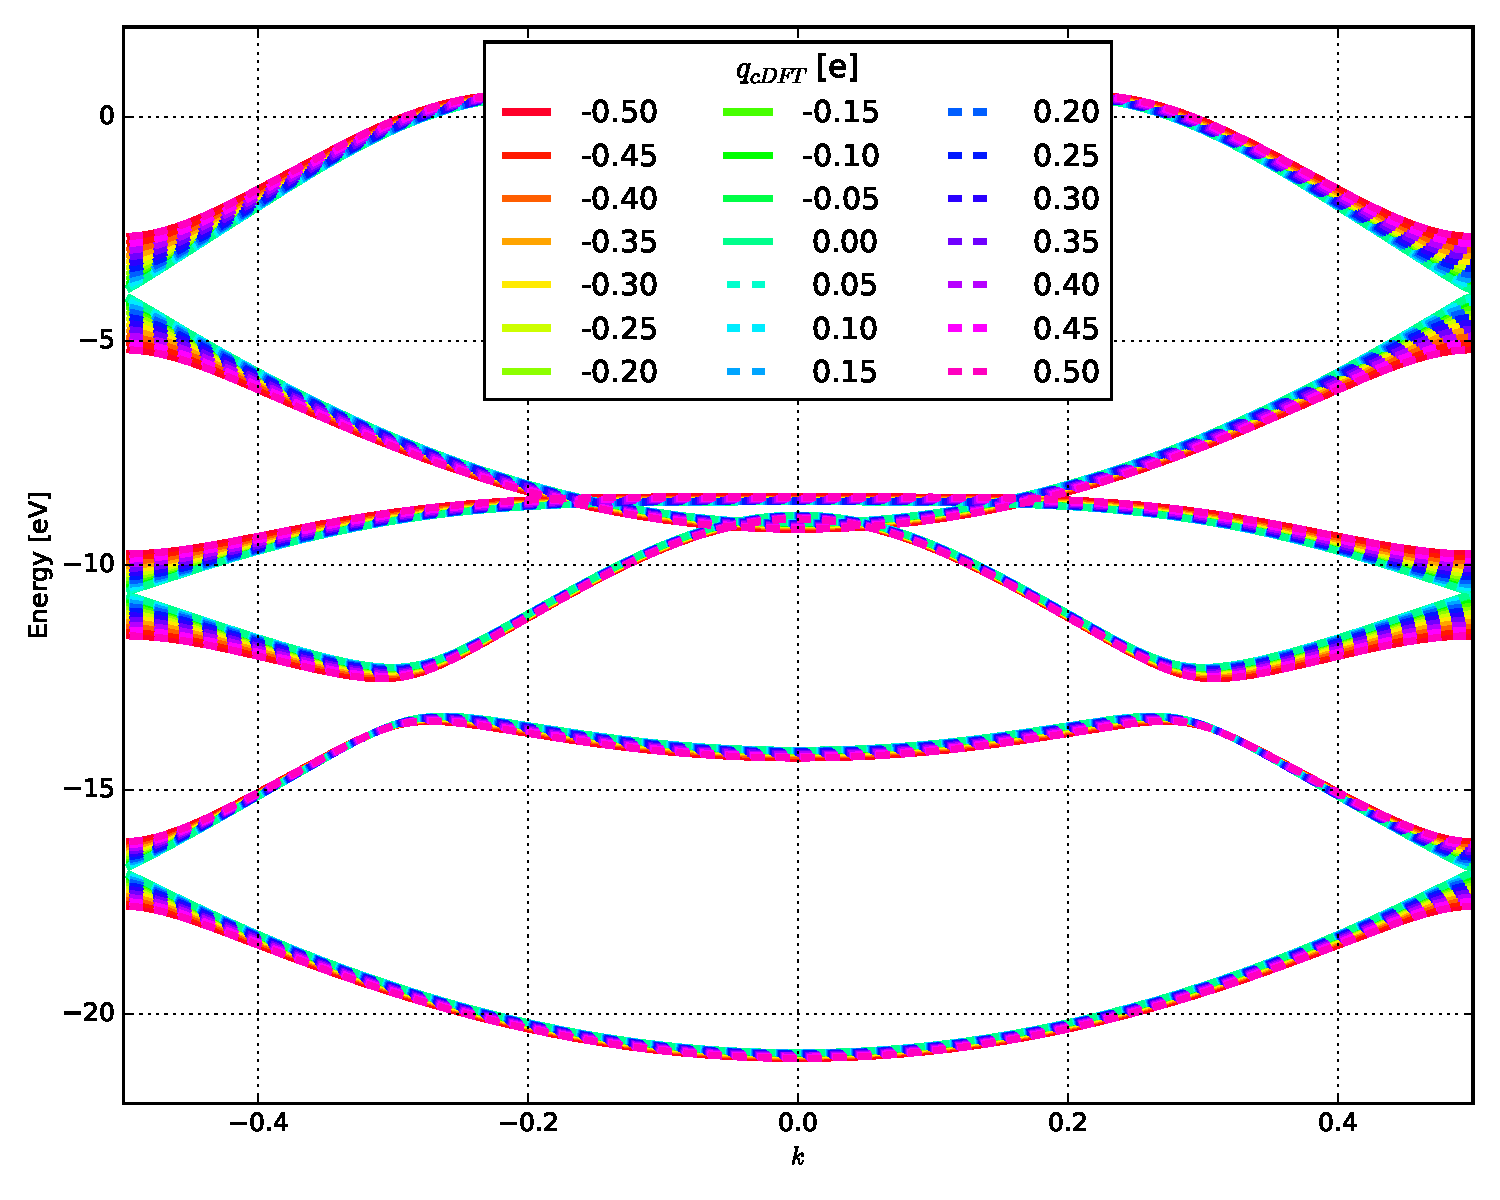
\includegraphics[width = 9.5cm]{Images/polyacetylene/charging/band_structure_q_1}
	\caption{Bandstruktur von \emph{trans}-Polyacetylen für verschiedene Ladungsverschiebungen.}
	\label{image_polyacetylene_band_structure_charging}
\end{figure}
\end{frame}

\begin{frame}
\begin{minipage}{0.49\textwidth}
	\begin{figure}
		\centering
		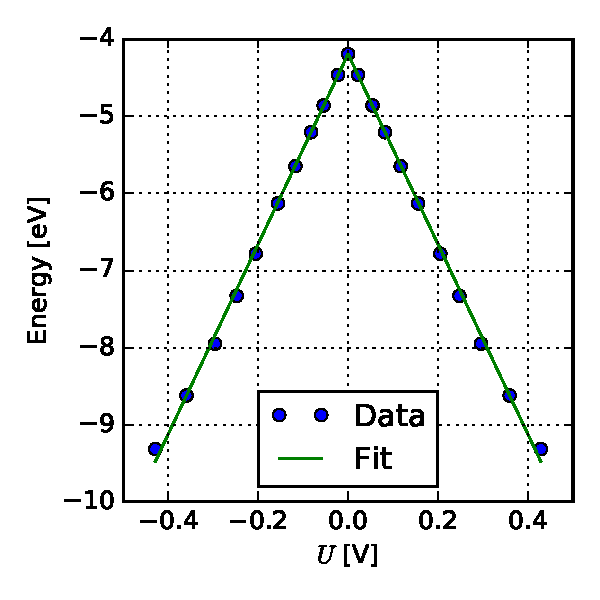
\includegraphics[width = \textwidth]{Images/Hydrogen/charging/border_energy_q_1}
		\caption{HOMO-Band-Energie am \textsc{Brillouin}-Zonen-Rand}
	\end{figure}
\end{minipage}
\begin{minipage}{0.49\textwidth}
	\begin{itemize}
		\setlength{\itemsep}{.5cm}
		\item Erwartete Bandform:
		\begin{align*}
		E_k &= - \sqrt{\left(cU\right)^2 + \left(2t_0\cos(ka)\right)^2}
		\end{align*}
		\item \textsc{Brillouin}-Zonen-Rand:
		\begin{align*}
		E_\text{Edge} &= -\left|cU\right|
		\end{align*}
		\item $c = \unit[12.3]{e}$
	\end{itemize}
\end{minipage}
\end{frame}

\begin{frame}
\begin{figure}
	\centering
	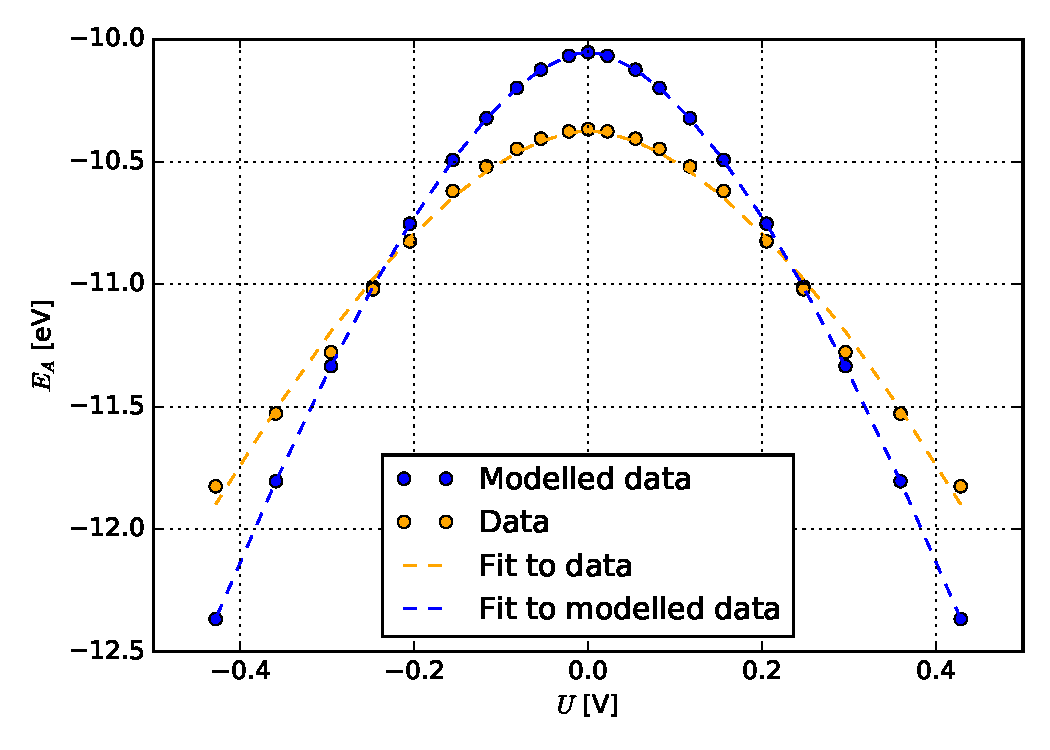
\includegraphics[width = 0.7\textwidth]{Images/Hydrogen/charging/Homo_energy_charge}
	\caption{Mittlere HOMO-Band-Energie in Abhängigkeit von $U$.}
\end{figure}
\begin{itemize}
	\item Daten: $\hspace*{1.9cm} t_0 = \unit[9.1]{eV}$
	\item Modellierte Daten: $t_0 = \unit[4.6]{eV}$
\end{itemize}
\end{frame}